\subsection{Components}

Figure \ref{fig:comp_dia} shows a high level view of the logical layout of the components in the MDApp.

\begin{figure}[H]
    \centering
    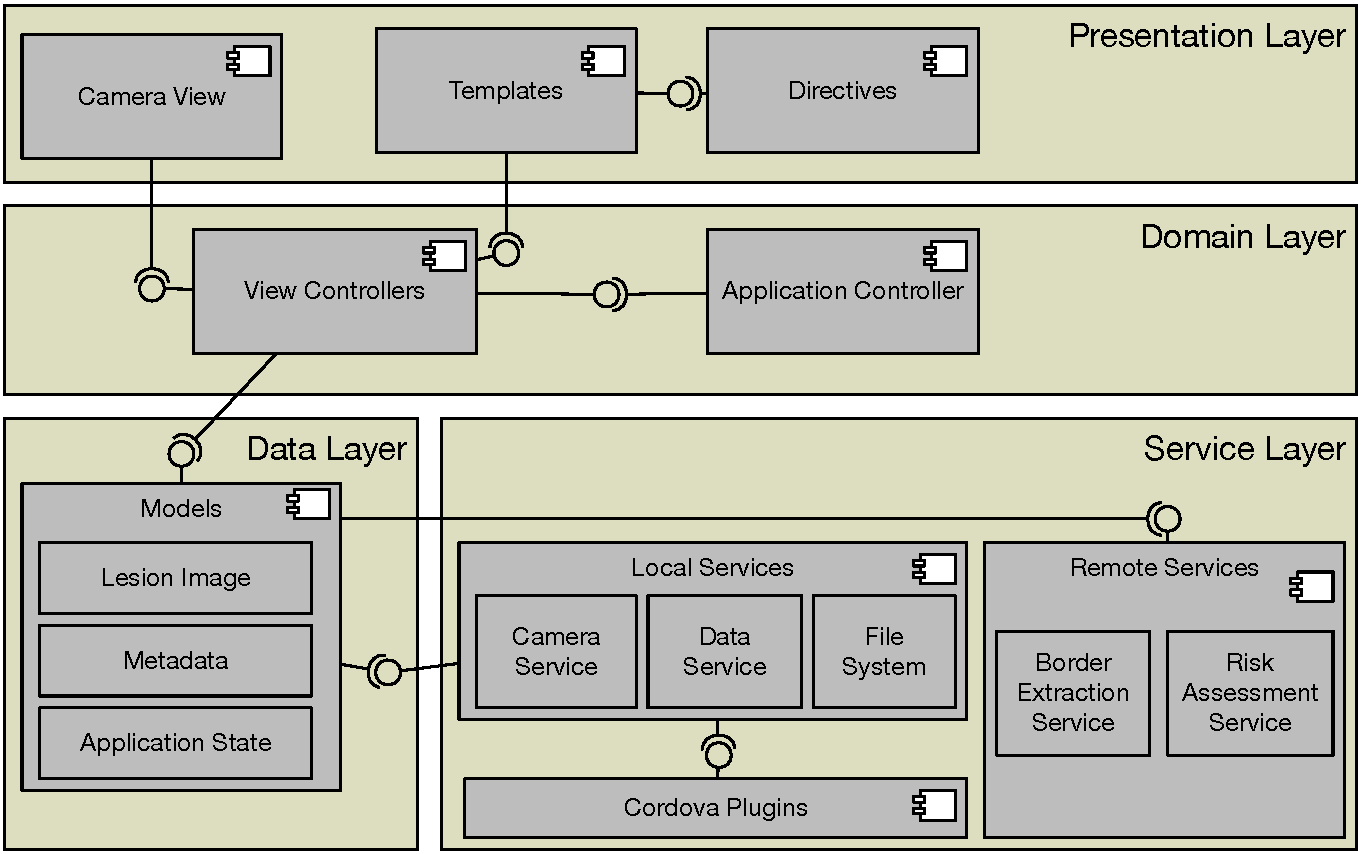
\includegraphics[width=\textwidth,keepaspectratio]{assets/architecture/compontent_diagram.pdf}
    \caption{Component diagram of the MDApp}
    \label{fig:comp_dia}
\end{figure}

\subsubsection{View Controllers}

Each view controller class is responsible for a specific view or partial view of the MDApp. In larger applications there might be multiple view controllers per “page” in a nested hierarchy. The MDApp will only require one controller per page, these are the HomeController, CameraController, AnalysisController and the ArchiveController. Each controller is responsible for preparing the data that will be displayed in the view as well as capturing and processing user events.

\subsubsection{Application Controller}
The application controller is a global controller that can manage the state of the app. It makes sure that the state is persevered when the MDApp is closed and restarted.


\subsubsection{Templates, Directives and Camera View}
Except for the the Camera View all of the pages are created from HTML files that have prepared placeholders called directives. Directives are special markers in the HTML that the Angular framework uses to inject data and specific behaviour into the HTML element. Directives bundle together often used patterns into easily configurable markers that can be embedded into an HTML file.

The Camera View is an exception in the MDApp. The CameraView is an HTML template that overlays a realtime preview of the camera’s input. The realtime preview is not part of the Cordova/Phonegap browser view, it is a platform native view element that is provided by a 3rd party plugin. The cordova-plugin-camera-preview is a crossplatofrm wrapper around native code that allows the browser based javascript to communicate and control the camera preview view.

\subsubsection{Models}


\subsubsection{Local Services}
\subsubsection{Remote Services}

\subsection{Classes}